%
% File: chap01.tex
% Author: Liam O'Shea
% Description: Introduction chapter where the boxing goes.
%
\let\textcircled=\pgftextcircled
\chapter{Implementation}
\label{chap:intro}

\initial{B}egging implementation chapter. How the hell do I start this. What even goes here.

%=======
\section{Comparison Methods}
\label{sec:sec01}


I began by plotting the initial Kinect Data over time in an attempt to understand \& visualise the nature of the data. I decided to use differentiation as a method of smoothing and to get the velocity data from distance.


\begin{figure}[t!]
\centering
\begin{minipage}{6.0cm}
    \centering
    \subtop[]{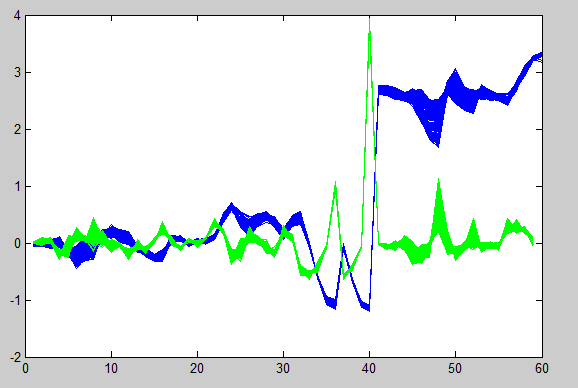
\includegraphics[height=0.25\textheight]{fig04/fig06}}
    \label{fig:1}
\end{minipage}
\begin{minipage}{6.0cm}
    \centering
    \subtop[]{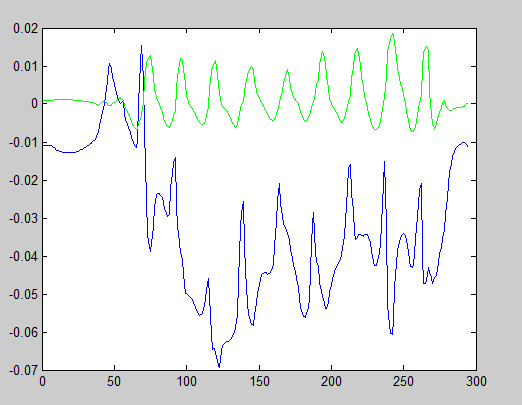
\includegraphics[height=0.25\textheight]{fig04/fig07}}
    \label{fig:2}
\end{minipage}
\mycaption[ALLData] {(a) Kinect Skeleton vs Time. 
(b) Hip Joint vs Time, Blue = Raw data, Green = Differentiated data.}
\end{figure}

After recording a punch sequence my first inclination was to look at the left hand (jab) over time. I plotted the z co-ordinate of the left wrist joint over each frame which produced a periodic pattern for which looked promising.


\begin{figure}[h]
    \centering
    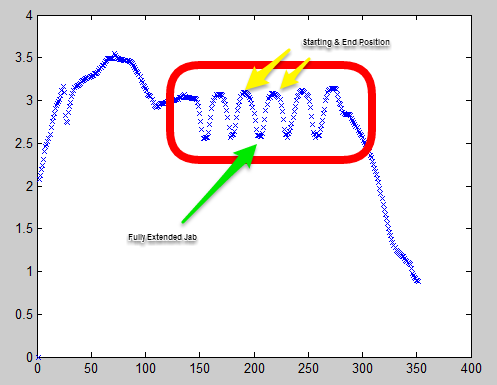
\includegraphics[height=0.25\textheight]{fig04/fig01}
    \mycaption[Kinect Device]{Depth of left wrist joint over time}
    \label{fig:kinect}
\end{figure}







My next step was punch segmentation. Due the clear cyclical nature of the punch movement I needed to develop a method for segmenting the punches. I decided the best way to do this was to smooth the signal and use local maxima/minima as a means of successfully segmenting the beginning and end of each punch. As you can see from Figure 4.2 some smoothing was required due to local maxima/minima which did not signify the beginning or end of a punch.



\begin{figure}[t!]
\centering
\begin{minipage}{6.0cm}
    \centering
    \subtop[]{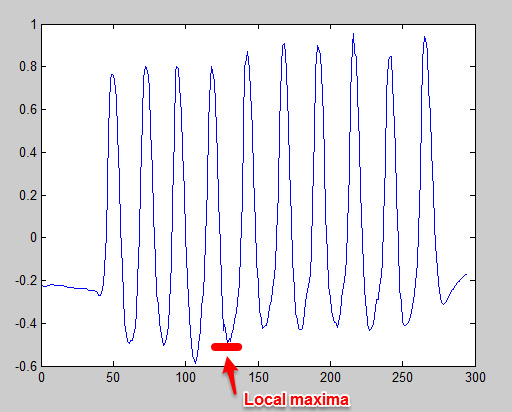
\includegraphics[height=0.25\textheight]{fig04/fig02}}
    \label{fig:kinect}
\end{minipage}

\hspace{0.5cm}
\begin{minipage}{6.0cm}
    \centering
    \subtop[]{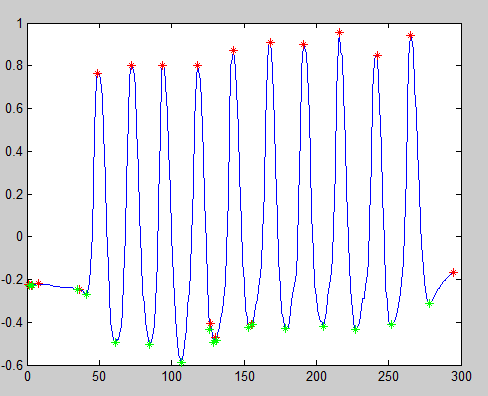
\includegraphics[height=0.25\textheight]{fig04/fig04}}
    \label{fig:kinect2}
\end{minipage}
\begin{minipage}{3.5cm}
    \centering
    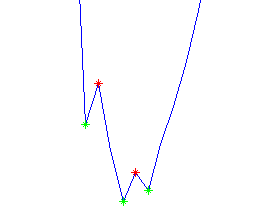
\includegraphics[height=0.15\textheight]{fig04/fig05}
    \label{fig:kinect3}
\end{minipage}
\mycaption[WAT]{(a) Periodic punch signal over time (frame number).(b) Periodic signal with local maxima/minima labelled. (c) Close up of local maxima/minima.}
\end{figure}


Smoothing.
I looked at using differentiation as a means of getting velocity and using that as a sensible measure to mark my punches. This did a good job of smoothing out the curve which would allow me to successfully segment my punches. 


\begin{figure}[h]
    \centering
    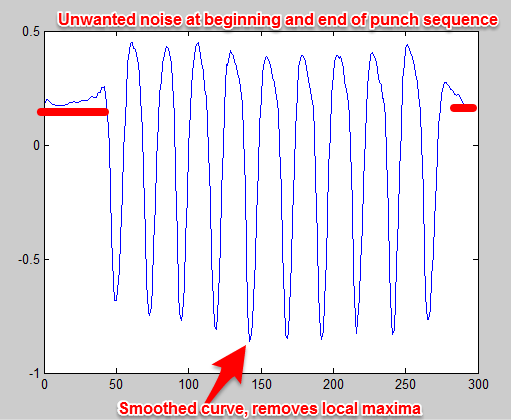
\includegraphics[height=0.25\textheight]{fig04/fig03}
    \mycaption[Kinect Device]{Depth of left wrist joint over time}
    \label{fig:kinect}
\end{figure}


Tested different dimensionality reduction techniques




{\bf Hidden Markov models?}
Svm?\newline
Chapter 3: Specification \& Design\newline
Scope Algorithms\newline
Chapter 4: Implementation\newline
Chapter 5: Data capture??\newline
Need to make and collect data consent forms to run a study?\newline
Need to gather more data?\newline

\paragraph{Data Format}
I record data from the Kinect in a space separated text file with each line corresponding to one timeframe. The structure of a line is: 
tracking_flag x_0 y_0 z_0 tracking_flag x_1 y_1 z_1 ... tracking_flag x_19 y_19 z_19,
where x_i,y_i,z_i are the x,y,z coordinates representing the position of the ith joint.
Each new line is represented by a very large value that could not represent a Kinect measurement. (e.g. 2000000) 
The tracking_flag is an integer which describes the status of the joint:
Joint not tracked = 0, Joint position inferred = 1, Join position tracked = 2.
If the joint is not tracked the position is set to (-10000, -10000, -10000) and it should not be used.
The position of the camera is (0,0,0).


The joints are:
i=0: NUI_SKELETON_POSITION_HIP_CENTER
i=1: NUI_SKELETON_POSITION_SPINE
i=2: NUI_SKELETON_POSITION_SHOULDER_CENTER
i=3: NUI_SKELETON_POSITION_HEAD
i=4: NUI_SKELETON_POSITION_SHOULDER_LEFT
i=5: NUI_SKELETON_POSITION_ELBOW_LEFT
i=6: NUI_SKELETON_POSITION_WRIST_LEFT
i=7: NUI_SKELETON_POSITION_HAND_LEFT
i=8: NUI_SKELETON_POSITION_SHOULDER_RIGHT
i=9: NUI_SKELETON_POSITION_ELBOW_RIGHT
i=10: NUI_SKELETON_POSITION_WRIST_RIGHT
i=11: NUI_SKELETON_POSITION_HAND_RIGHT
i=12: NUI_SKELETON_POSITION_HIP_LEFT
i=13: NUI_SKELETON_POSITION_KNEE_LEFT
i=14: NUI_SKELETON_POSITION_ANKLE_LEFT
i=15: NUI_SKELETON_POSITION_FOOT_LEFT
i=16: NUI_SKELETON_POSITION_HIP_RIGHT
i=17: NUI_SKELETON_POSITION_KNEE_RIGHT
i=18: NUI_SKELETON_POSITION_ANKLE_RIGHT
i=19: NUI_SKELETON_POSITION_FOOT_RIGHT

%=========================================================